\cotefile{43}
\scanpage{64}
% top product, with its lower identification
\[
\underbrace{\prod_{{\unsure{p|\mathfrak p}}_1\unsure{<|\backslash}p_2<\cdots<\text{\uline{\uuline{$p_n$}}}}
 A_{[p_1,p_2\unsure{-|,}p_n]}}_{{\unsure{\mathscr A|\mathcal A}}^{\unsure{n|u}}}
 \leftarrow \prod_{{\unsure{q|\mathfrak q}}_1<\cdots<q_{n-1}} A_{[q_1,\ldots,q_{n-1}]}
\]
\margin{\unsure{cosimplicial} ?!}
\[
p_1\supset p_2\supset\cdots\supset p_n
\]
\[
x_1\leq x_2\;\text{---}\;\leq x_n
\]
\figure{\begin{tikzpicture}[scale=.8]
\draw[<-] (0,0)--(3.4,-.3);
\draw (-.25,-.55)--(.05,.35) (.55,-.6)--(.75,.4) (2.7,-.65)--(3,.35);
\draw (5.3,1.25)--(5.35,1.05) (7.3,1.25)--(7.3,1.05);
\draw[->] (.2,.55)--(.7,.55); \draw (1.15,.55)--(1.4,.5) (2.3,.45)--(2.9,.45);
\end{tikzpicture}}
\[
A_{p,q}
\]
\figure{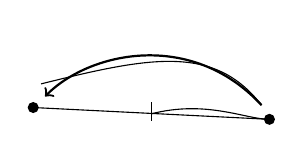
\begin{tikzpicture}
\fill (0,0) circle(2pt) (3,-.15) circle(2pt);
\draw (0,0)--(3,-.15); \draw (1.5,-.17)--(1.5,.07);
\draw[->,thick] (2.9,.03) .. controls (2,1) and (.7,.7) .. (.15,.14);
\draw (1.5,-.08) .. controls (2.2,.1) and (2.7,-.15) .. (3,-.15);
\draw (.1,.3) .. controls (1.5,.65) and (2.3,.8) .. (2.9,.03);
\end{tikzpicture}}
\[
\prod_{q<p} A_{[q,p]}\qquad \theta^2=0
\]
\figure{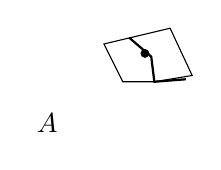
\begin{tikzpicture}[scale=.8]
\node at (-1.2,-.65) {$A$};
\draw (0,0)--(-.3,.6)--(.75,.85)--(1.1,.1)--(.5,0)--cycle;
\draw[thick] (.1,.7)--(.45,.4)--(.5,0)--(1,.04);
\fill (.35,.45) circle(2pt);
\end{tikzpicture}}
% middle, arrows and products
\diagram{\begin{tikzcd}[ampersand replacement=\&,column sep=large,row sep=large]
{}\& {\sum1_{q,p}} \arrow[l,bend right=12] \arrow[ddr,bend left=65] \& \\
{} \& {[p_1\supset\cdots\supset p_n]} \arrow[l] \arrow[d,"1_{qp}"] \arrow[dl,"{\unsure{\coprod}}_{q}1_{q,p_1}"'] \& \\
{\prod_q [q\supset p_1\supset\cdots\supset p_n]} \& {} \& {\prod_q[p_1\supset\cdots\supset p_n\supset q]}
\end{tikzcd}}
\figure{\begin{tikzpicture}
\draw[<-] (0,0)--(3.1,0);
\draw (0,.9) .. controls (0,.5) and (1,.6) .. (1.5,.7) .. controls (2,.9) and (2.2,.1) .. (3.2,.5);
\draw (1.2,2.1) .. controls (1,2.5) and (1.7,2.6) .. (2.1,2.4) .. controls (3,2.1) and (4,2.5) .. (4.2,1.9);
\draw[<-] (3.6,2)--(4.2,2);
\end{tikzpicture}}
\par\noindent\rule{\linewidth}{.4pt}
% lower notes
\[
A_{[p_1,\ldots,p_r]}
\]
\margin{$\unsure{\widehat A_p/p\widehat A_q|\widehat A_q/p\widehat A_q}$}
\unsure{anneau local} \unsure{muni} de $r$ topologies (\unsure{non adiques en général}) \unsure{différentes}, ${\unsure{T|\mathbb T|\Pi}}_1,\ldots,T_r$ (\unsure{pas nécessairement compatibles}) \unsure{métrisables} \deleted{\unsure{séparées}} et \unsure{complètes}.
\margin{$\widehat A_q$}
\figure{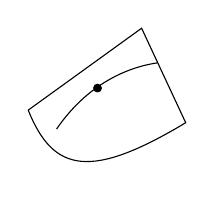
\begin{tikzpicture}[scale=.8]
\draw (0,.1)--(1.8,1.4)--(2.5,-.1) .. controls (1,-1) and (.4,-.9) .. (0,.1);
\draw (.45,-.2) .. controls (1,.6) and (1.7,.8) .. (2.05,.85);
\fill (1.1,.45) circle(2pt);
\end{tikzpicture}}
\unsure{Un} \unsure{germe} \unsure{filtré} \unsure{tend} vers $0$ pour $T_i$, \unsure{à} \unsure{fond} et \unsure{uniformément} \unsure{pour} \unsure{pour} $\forall$ voisinage de $0$ $V_{i+1}$ pour $T_{i+1}$,
% archive sheet number: 65
